\chapter{An Overview on Software Product Lines and CASE tools}
\label{ch:background}

\begin{quotation}[John Calt]{Dreams Come Due}
Believe nothing, no matter where you read it, or who said it, no matter if I have said it, unless it agrees with your own reason and your own common sense
\end{quotation}


\ac{SPL} has proven to be a successful approach in many business environments \citep{clements2002software}. Moreover, it is an interesting methodology for developing a diversity of software products and software-intensive systems at lower costs, in shorter time, and with higher quality \citep{Pohl2005}. Product line engineering comprises many heterogeneous activities such as capturing the variability of reusable assets, supporting the derivation of products from the product line, evolving the product line, or tailoring the approach to the specifics of a domain. The inherent complexity of product lines implicates that tool support 
is inevitable to facilitate smooth performance and to avoid costly error \citep{Dhungana2007}.CASE tools may greatly assist on maintain an efficient \acf{SPL} process, automatizing tasks, keeping traceability links and dealing with variability.

Based on the context of this work and the importance of \acf{CASE} tools on a \acf{SPL} lifecycle management, this chapter concerns the understanding of two important topics for this dissertation: Software Product Lines and \ac{CASE} tools. \secref{sc:productlines} discusses \acf{SPL}, its characteristics, development processes and benefits. 

\secref{sc:casetools} explains the \ac{CASE} Tools it applications and benefits. Recently, the term \acf{ALM} had appeared in the literature, and “has emerged to indicate the coordination of activities and the management of artifacts (e.g. requirements, source code, test cases) during the software product's lifecycle” \citep{Jukka:2009} , and we also provide a brief overview about \ac{ALM}.\secref{sc:relatedWork} addresses the what was been proposed in the literature and tools available in the market. Finally, \secref{sc:summary} presents a summary of this Chapter.



\section{Software Product Lines}
\label{sc:productlines}

\subsection{Introduction}
Nowadays, we are living in the age of customization. The customer want to have the ability to demand products that specifically address their segment or, sometimes, customer-specific adaptations to their software's \citep{rafael2013systems}.  

In today fast-paced world, companies cannot afford the luxury of not hearing what the market is asking for, and because of that, many companies have found the notion of software product lines. \acf{SPL} provide a set of work practices that allows them to drastically increase the amount of R\&D resources that focused on highly differentiating functionality and, consequently, decreasing the investment in commoditized functionality. 

A \ac{SPL} is outlined as a collection of similar software intensive systems that share a set of common features satisfying the wants of specific customers, market segments or mission. Those similar software systems are developed from a set of core assets, comprised of documents, specifications, components, and other software artifacts that may be reusable throughout the development of each system within the product line \citep{rafael2013systems}.

 \acf{SPL} is concerned with sharing common functionality within a family of products. Earlier approaches to software reuse had a tendency to focus only on the technology aspects of reusing software assets and occasionally included some process aspects. According to \citep{rafael2013systems}. Some factors that make software product lines successful is that it addresses business, architecture, process and organizational aspects of effectively sharing software assets within a portfolio of products. 


\begin{figure}[htp]
\begin{center}
  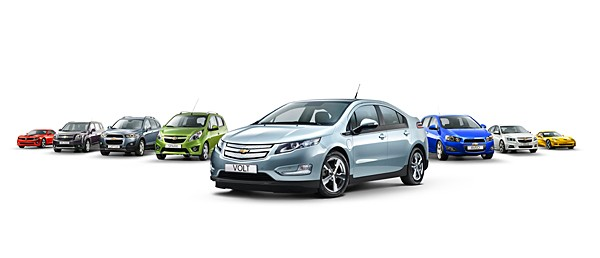
\includegraphics[width=9cm]{chapters/background/img/chev-line.jpg}
  \caption[Chevrolet Product Line]{Chevrolet Product Line.}
  \label{fg:chev-line}
\end{center}
\end{figure}


One example is General Motors , the largest automotive manufacturer in the world \citep{GmTop2012}. In 2011 it sold over nine million vehicles, produced (with its partners) in 31 countries around the world. Producing over than 1,000 vehicles off their assembly lines every hour \citep{rafael2013systems}. \figref{fg:chev-line} depicts a General Motors company and their product line of cars.


\subsection{The Benefits}

Successful introduction of a software product line provides a significant opportunity for a company to improve its competitive position \citep{rafael2013systems} , and according to \citep{ clements2002software,Pohl2005, rafael2013systems} many benefits can be identified, some examples follow:
\begin{itemize}

\item \textbf{Product portfolio diversity}

The primary and possibly most popular reason for introducing a software product line is to be able to offer a much broader and richer product portfolio against the same R\&D investment. Particularly in the case where the market is currently served by a small number of independently developed products, and can be more effectively monetized by offering more products serving smaller customer segments. More accurately, the introduction of the product line allows for effective sharing of functionality needed by all products while allowing for product-specific functionality being built on top to serve the specific market segment. \citep{rafael2013systems}.



\item \textbf{Cost reduction}

One good motive for introduce new software product line is the reduction in costs. Those reductions can come from the reuse of artifacts between a number of different systems, as is saving work to create and maintain the artifacts to each product. However, before those artifacts can be used, it should be created in a way to possibility this use, and this do not come free. This means that the company has to make an up-front investment to create the platform before it can reduce the costs per product by reusing platform artifacts.

\begin{figure}[htp]
\begin{center}
  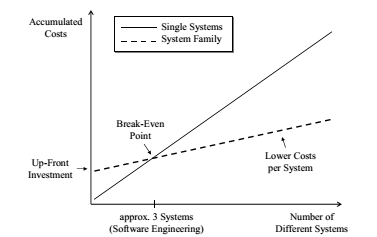
\includegraphics[width=11cm]{chapters/background/img/splcosts.png}
  \caption[Costs for developing systems as single systems compared to product 
  line engineering]{Costs for developing systems as single systems compared to product line engineering \citep{Pohl2005}}
  \label{fg:spl-costs}
\end{center}
\end{figure}

\figref{fg:spl-costs} shows the built up costs required to develop a number of different systems. The solid line sketches the costs of developing the systems independently, while the dashed line shows the costs for product line engineering. In the case of a few systems, the costs for product line engineering are relatively high, whereas they are significantly lower for larger quantities. The location at which both curves intersect marks the break-even point. At this point, the costs are the same for developing the systems separately as for developing them by product line engineering. The precise location of the break-even point depends on various characteristics of the organization and the market it has envisaged such as the customer base, the expertise, and the range and kinds of products \citep{Pohl2005}.

\item \textbf{Quality improvement}


The use of a \acf{SPL} can also bring an improvement in the overall quality of all artifacts.

A quite typical, but less publicized, alternative reason for introducing a software product line is to share one major subsystem between the products in the portfolio. One example is to share the UI framework and the generic menu structure and use cases between the products. This allows for a common look and feel across the product portfolio allowing for higher productivity of users that use different devices from the same manufacturer \citep{rafael2013systems}.

Creating the products from shared components and based on a common architecture means that the artifacts in the platform are reviewed and tested in many products. They have to prove their proper functioning in more than one kind of product. The extensive quality assurance indicates a significantly higher opportunity of detecting faults and correcting them, thereby improving the quality of all products \citep{Pohl2005}.


\begin{figure}[htp]
\begin{center}
  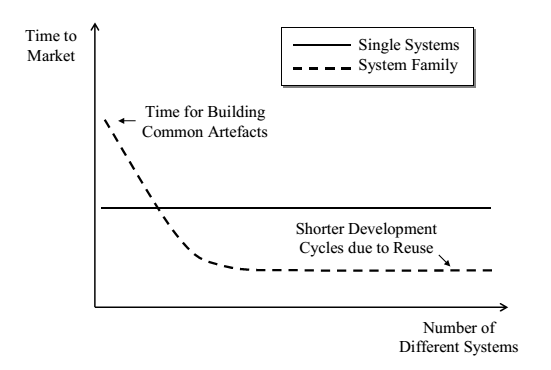
\includegraphics[width=11cm]{chapters/background/img/spl-timetomarket.png}
  \caption[Comparison of time to market with and without product line engineering]{Comparison of time to market with and without product line engineering}
  \label{fg:spl-timetomarket}
\end{center}
\end{figure}

\item \textbf{Reduction of time-to-market}


Another very important success factor for a product is the time to market.  For developing a single-product, you could do faster, in a constant time. For developing a \acf{SPL} you have an entry barrier and the time to market indeed is initially higher as the common artifacts have to be built first. However after the initial  hurdle, the time to market is considerably shortened as many artifacts can be reused for each new product, as can be seem on \figref{fg:spl-timetomarket}




\end{itemize}


\subsection{The SPL Development Process}

The \acf{SPL} Development Process has a number of definitions depending on the author. Two popular definitions on the literature \citep{clements2002software,Pohl2005} have similar interpretations that can be related to each other. \citet{clements2002software} defined three essential activities to Software Product Lines: \textbf{\acf{CAD}} activity that aims to develop assets to be further reused in other activities; \textbf{\acf{PD}} activity, which takes advantage of existing, reusable assets and \textbf{Management} activity, which includes technical and organizational management. \figref{fg:spl-activities} illustrate those activities. In addition \cite{Pohl2005} defined a framework for software product line engineering composed of two processes:

\begin{figure}[htp]
\begin{center}
  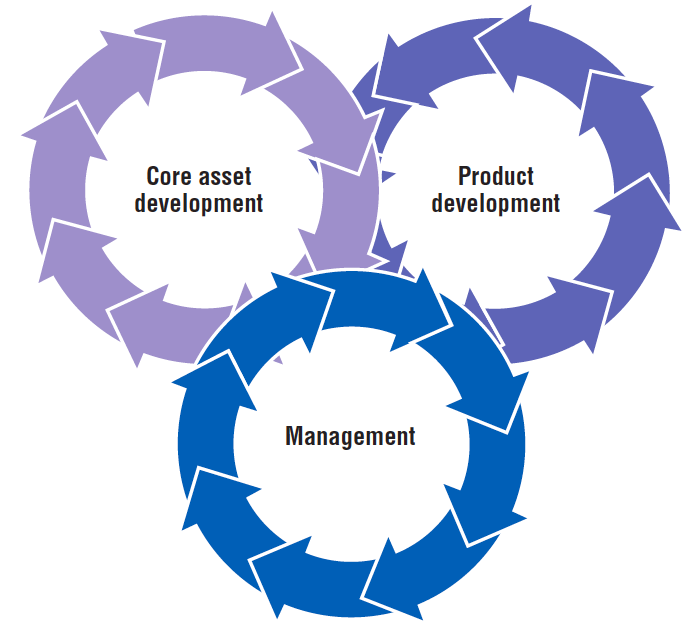
\includegraphics[width=10cm]{chapters/background/img/SPLactivities.png}
  \caption[SPL Activities]{SPL Activities \citep{clements2002software}}
  \label{fg:spl-activities}
\end{center}
\end{figure}


\begin{itemize}
\item \textbf{Domain engineering:} This process is responsible for establishing the reusable platform and thus for defining the commonality and the variability of the product line.
\item \textbf{Application engineering:} This process is responsible for deriving product line applications from the platform established in domain engineering;
\end{itemize}
An Overview of this framework can be seen in \figref{fg:spl-pohlframework}.  In essence those two approaches are related, where  \acf{CAD} activity is the Domain engineering process, and the \acf{PD} activity is the Application engineering process. Lastly, the management activity control the execution of the whole process. 





\begin{figure}[htp]
\begin{center}
  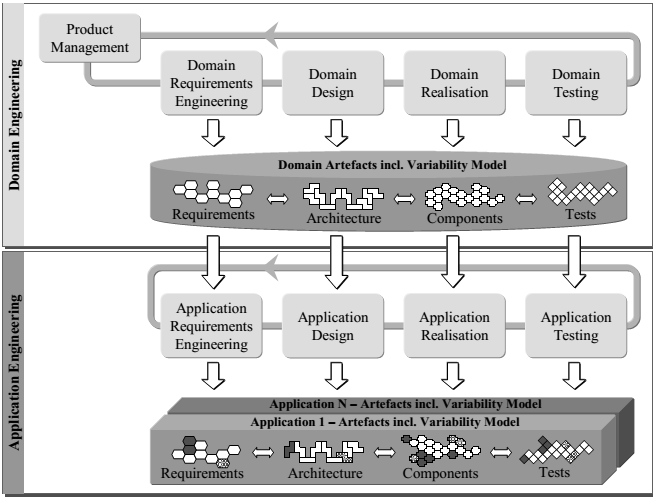
\includegraphics[width=13cm]{chapters/background/img/pohl-framework.png}
  \caption[The software product line engineering framework]{The software product line engineering framework \citep{Pohl2005}}
  \label{fg:spl-pohlframework}
\end{center}
\end{figure}





\subsubsection{Core Asset Development}


\acf{CAD}, also called by \citep{Pohl2005} as \textit{domain engineering}, it’s an activity that results in the common assets that in conjunction compose the product line’s platform \citep{clements2002software}.The key goals of this activity are \citep{Pohl2005}:
\begin{itemize}
\item Define the commonality and the variability of the software product line.
\item Specify the set of applications the software product line is planned for.
\item Determine and construct reusable artifacts that accomplish the desired variability.
\end{itemize}

In \figref{fg:spl-coreasset}, is shown the core asset development activity. This activity is interactive, and its inputs and outputs influence each other. The inputs includes product constraints; production constraints; architectural styles; design patterns; application frameworks; production strategy and preexisting assets. 
This phase is composed of the sub processes as follow \citep{Pohl2005}: 
\begin{itemize}

\item \textbf{Product Management} deals with the economic aspects associated with the software product line and in particular with the market strategy.
\item \textbf{Domain Requirements Engineering} involves all activities for eliciting and documenting the common and variable requirements of the product line.
\item \textbf{Domain Design} encompasses all activities for defining the reference architecture of the product line, 
\item \textbf{Domain Realization} deals with the detailed design and the implementation of reusable software components.
\item \textbf{Domain Testing} is responsible for the validation and verification of reusable components. 
\end{itemize}

\begin{figure}[htp]
\begin{center}
  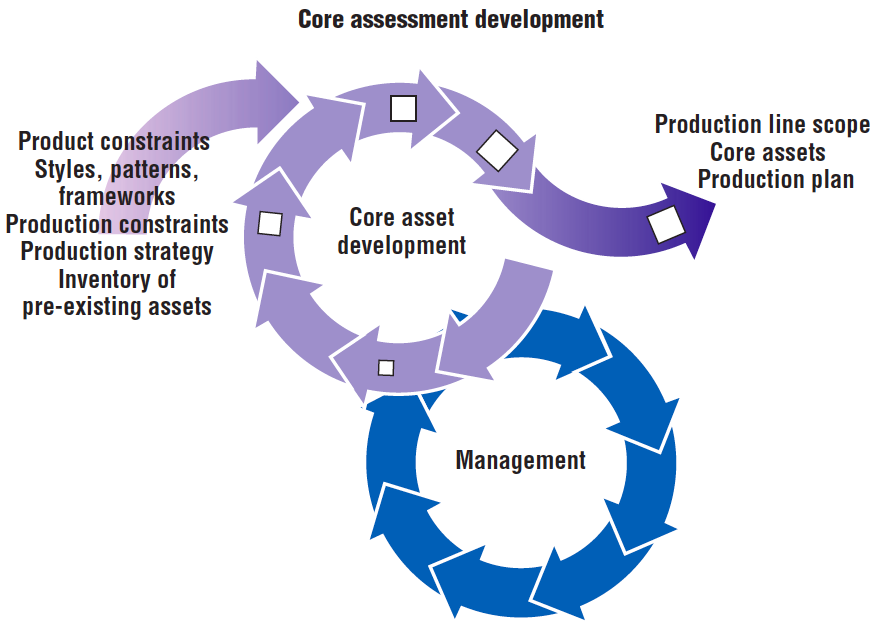
\includegraphics[width=10cm]{chapters/background/img/SPLcoreasserts.png}
  \caption[Core Asset Development]{Core Asset Development \citep{clements2002software}}
  \label{fg:spl-coreasset}
\end{center}
\end{figure}

This activity have three outputs: \textbf{Product Line Scope}, \textbf{Core Assets} and \textbf{Production Plan}. The first output, \textit{Product Line Scope}, describes the products that will constitute the product or that the product line is capable of including. Although this description can be as simple as an enumerated list, it is preferred to be detailed and carefully specified, for example, including market analysis activities in order to determine the product portfolio and to encompass which assets and products will be part of the product line. This specification must be driven by economic and business reasons to keep the product line competitive \citep{rafael2013systems}.

\textit{Core assets} are the basis for production of products in the product line. It includes an architecture that will fulfill the needs of the product line, specify the structure of the products and the set of variation points required to support the spectrum of products. It may also include components and their documentation \citep{clements2002software}.

Lastly, the \textit{production plan} describes how products are produced from the core assets. It details the overall scheme of how the individual attached processes can be fitted together to build a product \citep{clements2002software}. It is what link all the core assets together, guiding the product development within the constraints of the product line.




\subsubsection{Product Development}

\begin{figure}[htp]
\begin{center}
  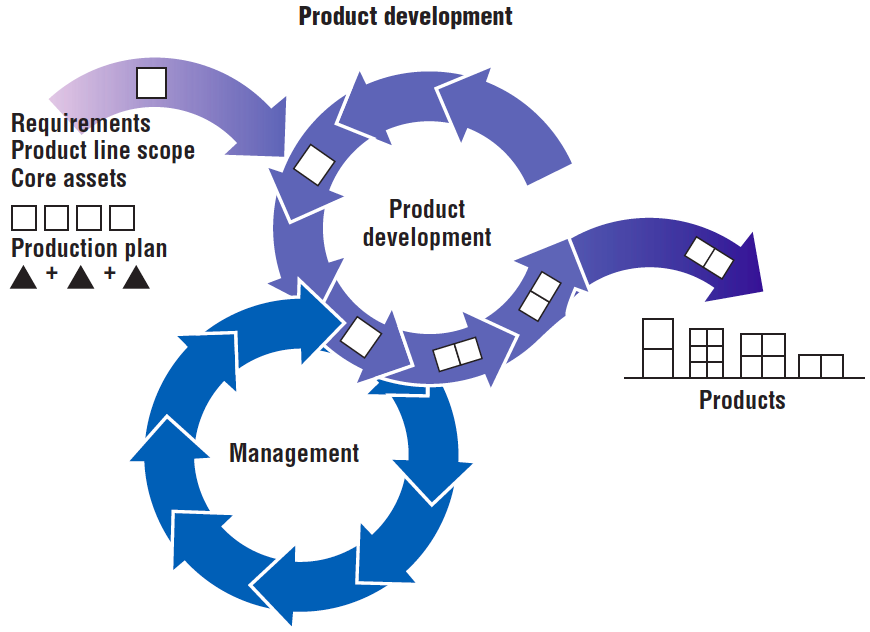
\includegraphics[width=10cm]{chapters/background/img/SPLproduct-development.png}
  \caption[Product Development]{Product Development \citep{clements2002software}}
  \label{fg:spl-productdev}
\end{center}
\end{figure}


The production plan \figref{fg:spl-productdev}, will detail how the core asserts can be used to build a product, and will be used to assemble individual product line members. The inputs for this activity are the artifacts built in the core assets development activity (product line scope, core assets, and production plan) and the requirements specification for individual products.

The outputs from this activity should be analyzed by the software engineer and the corrections must be feed back to the \acf{CAD} activity. During the product development process, some insights happens and it is important to report problems and faults encountered to keep the core asset base healthy.



\subsubsection{Management}

The management activity is responsible for the production strategy and is vital for success of the product line \citep{Pohl2005}. It is performed in two levels: technical and organizational. The technical management supervise the CAD and PD activities by certifying that both groups that build core assets and products are focused on the activities they supposed to, and follow the process. The organizational management must ensure that the organizational units receive the right resources in sufficient amounts \citep{clements2002software}.

\section{CASE Tools}
\label{sc:casetools}
\acf{CASE} tools aim to support software engineering process activities. These tools provide process support by automating some process activities and by providing information about the software that is being developed, allowing them to develop high quality systems, easy maintained and reliable (Albizuri-Romero, 2000). Their usage is greatly growing lately, because the current sophistication in SE processes means that they are hard to accomplish without reasonable tool support \citep{Dhungana2007}.

\subsection{Benefits of CASE tools}

\begin{itemize}
\item Improved communications: The communications seems to be enhanced both between project engineers and customer and among engineers working on a project;
 \item Improved documentation: The documentation improvement relates to a greater consistency and accuracy in specifying the system and in the direct generation of portions of the documentation by the CASE tools.
\item Facilitate update and modification of diagrams: The lack of tool support executing in this task makes it time consuming and difficult, and can, eventually, lead to problems in the documentation produced.
\item Assist method institutionalizing: Companies aim at achieving a more standardized way of performing software development. For that, they need a better process structure through a wider use of methods that can be easily followed. Thus, tools focused on processes (Process-Centered Software Engineering Environments -PSEE) can secure the methods rules, which can guide to an easier maintenance process.
\item Achieve a faster dialog with customers/end-users: The conversation with the customers/end-user about the product requirements, usually occur through documents and diagrams. With the tools, the manipulation of these documents/diagrams becomes faster and easier, increasing the dialogs with the customers/end-user. 

\item  Increase the work flexibility: The companies’ motivation to use CASE was the possibility of easily modifying the development methodology according to the specific situation of the product to be developed.

\item  Improve documentation: Through the improvement in documentation, companies achieve not only an easier product to maintain, but it also improves product's comprehension during customer/end-users conversations. Another motive given by the companies is that they want to improve the development reports.

\item  Reduce working effort: The tools can be useful for saving working time in routine work products, leaving more time to focus in improving the product's quality.

\end{itemize}


\subsection{Application Lifecycle Management}

The development of software products is an extremely complex undertaking, consisting of numerous interdependent activities, various different roles and a wide range of artifacts spanning over all phases of the development project and across the whole product's lifecycle \citep{lacheiner2011}. 

In the past few years, the concept of \acf{ALM} has emerged with the objective to provide a comprehensive technical solution for monitoring, controlling and managing software development over the whole application lifecycle. \citep{Schwaber2006} defines \ac{ALM} as:

“The coordination of development lifecycle activities, including requirements, modeling, development, build and testing, through: 1) enforcement of processes that span these activities; 2) management of relationships between development artifacts used or produced by these activities; and 3) reporting on progress of the development effort as a whole.” Consequently tool vendors emphasize the move towards integrated tool suites \citep{lacheiner2011}.

The \ac{ALM} as a concept is quite new and there are many conflicting definitions on what constitutes \ac{ALM}, making the whole concept of ALM is unclear and driven by tool vendors. However, \citep{kaariainen2011towards} provides a framework for \ac{ALM} that outlines what a solid process must look like.


\begin{figure}[htp]
\begin{center}
  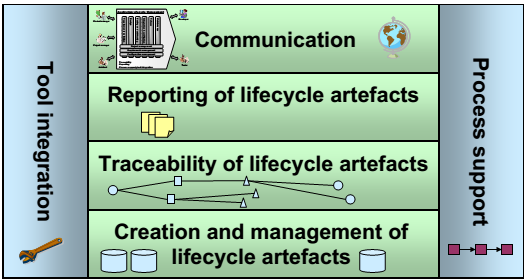
\includegraphics[width=10cm]{chapters/background/img/alm-framework.png}
  \caption[ALM Framework]{ALM Framework \citep{kaariainen2011towards}}
  \label{fg:alm-framework}
\end{center}
\end{figure}

\cite{kaariainen2011towards} came with the \ac{ALM} Framework presented on \figref{fg:alm-framework}. The elements in the middle form the levels of the \ac{ALM} elements (hierarchy) with the upper element using artifacts provided by the lower level elements. The role of process support and tool integration at the side provide an efficient working environment by equipping the elements presented in the middle to support an overall lifecycle process and tool integration. A brief description of each block, follows, \citep{kaariainen2011towards}:

\begin{itemize}

\item  \textbf{Creation and management of lifecycle artifacts} is the foundation of ALM. The product information collected and managed by this element is important for many reasons such as traceability and reporting activities.
\item  \textbf{Traceability of lifecycle artifacts} provides a means to identify and maintain relationships between lifecycle artifact, facilitating reporting, enabling change impact analysis and information visibility through the development lifecycle. 
\item  \textbf{Reporting of lifecycle artifacts} utilizes managed lifecycle artifacts and traceability information to generate needed reports from the lifecycle product information to support SW development and management. 
 \item  \textbf{Communication} enables communication tools (e.g., chat) as well as channels for distributing information on product lifecycle artifacts, links and reports and thus facilitates product information visibility for the whole \ac{SW} project. 
\item  \textbf{Process support and Tool integration} are the elements used to configure the \ac{ALM} solution to support \ac{SW} development procedures and facilitate a productive development environment by allowing the user to launch tools and transfer information easily between different tools and databases.

\end{itemize}

The \acf{SPLICE} tool developed in this work, can be considered not just a \ac{CASE} tool but, with reservations, a \acf{ALM} tool.

There are reports of \acf{ALM} tools been used to manage the Product Line engineering with  efficiency improvement, shorter lead time, and better quality in product development


\section{Tools Comparison}
\label{sc:relatedWork}

We conducted an informal search for similar commercial or academic tools. The search methodology consisted on searches on Google \footnote{http://www.google.com}, SourceForge \footnote{http://www.sf.net}, GitHub \footnote{http://www.github.com} and digital libraries of the most famous publishers and organizations in software engineering, ACM Digital Library and IEEE Computer Society Digital Library for the terms: 

\textit{“Project management”}, \textit{“Project management tool”}, \textit{“SPL project management”} and \textit{“Application Lifecycle Management”}. 

We also asked some of experts of the RiSE group, about tools they knew or heard about that would suit the task, and used the list of nineteen SPL tools compiled from the \cite{lisboa:msc:2008} thesis.

Initially we came up with \textbf{221} possible tools, and filtered using the include criteria that the tool must at least cover two areas of the \ac{SPL} process, like Requirements, Planning, Configuration management, Testing or Scoping. After the analysis, \textbf{twenty-three} tools were selected.

After the tool selection, we elected fourteen characteristics and functionalities that is interesting to be covered in an Application lifecycle tool. Table \ref{table:functionalitiestools} details which functionalities each tool offers support. The roman numbers refer to the functionalities that are described next. This table facilitates the identification of the gaps in the selected tools, and in addition it can help discovering which tool best satisfies a company’s needs.


\noindent\textbf{i) Commercial Tool}: represents if the tool is freely available, or a license is need.
\\
\\
\textbf{ii) Requirements}: provides support to include the requirements and/or use cases in the tool.
\\
\\
\textbf{iii) Agile Planning}: identifies if the tool provide support for planning using agile methodologies. 
\\
\\
\textbf{iv) Version Control Integration}: analyses if it provide integration and support for any \acf{VCS}.
\\
\\
\textbf{v) Issue Tracking}: verifies if the tool can manage issue reports. 
\\
\\
\textbf{vi) Testing}: identifies if the tool have support for activities or assets related the testing.
\\
\\
\textbf{vii) Scoping}: determines if the tool have the \textit{Feature} asset or something similar.
\\
\\
\textbf{viii) Traceability}: relates to the tool ability to provide traceability among the managed assets. 
\\
\\
\textbf{ix) Metamodel Customization}: analyses the possibility of changing and modeling the tool metamodel to specific needs. 
\\
\\
\textbf{x) Collaborative Documentation}: verifies if the tool have support for collaborative documentation such as \textit{Wikis}.
\\
\\
\textbf{xi) Web-based}: identifies if the tool have an interface that can be accessed online, or is a Desktop only product. 
\\
\\
\textbf{xii) Reports generation}: analyses if the tool can provide any kind of reports for the assets that it manages.
\\
\\
\textbf{xiii) Open-source}: specifies if the tool have the source-code publicly available.
\\
\\
\textbf{xiv) SPL oriented}: identifies if the tool is prepared or have features oriented specifically to the \ac{SPL} process.

\newcommand*\rot{\rotatebox{90}}

\begin{landscape}
\begin{table}[!ht]
\centering
\small
\tabcolsep=0.11cm
\begin{center}
    \begin{tabular}{|l|l|l|l|l|l|l|l|l|l|l|l|l|l|l|}

    \textbf{Functionalities / Tools}                         & \rot{Commercial Tool} & \rot{Requirements} & \rot{Agile Planning} & \rot{Version Control Integration} & \rot{Issue Tracking} & \rot{Testing} & \rot{Scoping}  & \rot{Traceability} & \rot{Metamodel Customization} & \rot{Collaborative Documentation} & \rot{Web-based} & \rot{Reports generation} & \rot{Open-source} & \rot{SPL oriented} \\ \hline
    BigLever  Gears           & Yes             & Yes          & No             & No                          & No             & No      & Yes            & Yes          & Partially               & No                          & No        & Yes                & No          & Yes          \\ \hline
    IBM Jazz                  & Yes             & Yes          & Yes            & Yes                         & Yes            & Yes     & Yes            & Yes          & Yes                     & No                          & Yes       & Yes                & No          & No           \\ \hline
    Polarion ALM              & Yes             & Yes          & Yes            & No                          & Yes            & Yes     & No SPL support & Yes          & Yes                     & Yes                         & Yes       & Yes                & No          & No           \\ \hline
    codeBeamer  ALM           & Yes             & Yes          & Yes            & Yes                         & Yes            & Yes     & No SPL support & Partially    & No                      & Yes                         & Yes       & Yes                & No          & No           \\ \hline
    Endeavour Agile ALM       & No              & Yes          & Yes            & Yes                         & Yes            & Yes     & No SPL support & Partially    & No                      & Yes                         & Yes       & Yes                & Yes         & No           \\ \hline
    FogBugz                   & Yes             & No           & Yes            & Yes                         & Yes            & No      & No             & No           & No                      & Yes                         & Yes       & Yes                & No          & No           \\ \hline
    FusionForge               & No              & No           & No             & Yes                         & Yes            & Yes     & No             & No           & No                      & Yes                         & Yes       & No                 & Yes         & No           \\ \hline
    Gemini Tracker            & Yes             & No           & Yes            & Yes                         & Yes            & No      & No             & No           & No                      & No                          & Yes       & Yes                & No          & No           \\ \hline
    Parasoft Concerto         & Yes             & Yes          & Yes            & No                          & Yes            & Yes     & No             & Yes          & No                      & No                          & Unknown   & Yes                & No          & No           \\ \hline
    Visual Studio TFS         & Yes             & No           & Yes            & Proprietary                 & Yes            & Yes     & No             & No           & No                      & No                          & No        & Yes                & No          & No           \\ \hline
    Workspace.com             & Yes             & Yes          & No             & No                          & Yes            & Yes     & No             & No           & No                      & Yes                         & Yes       & No                 & No          & No           \\ \hline
    Rally ALM                 & Yes             & Yes          & Yes            & No                          & Yes            & Yes     & No             & No           & No                      & Yes                         & Yes       & Yes                & No          & No           \\ \hline
    Redmine                   & No              & No           & Plugin         & Yes                         & Yes            & No      & No             & No           & No                      & Yes                         & Yes       & Yes                & Yes         & No           \\ \hline
    Trac                      & No              & No           & Plugin         & Yes                         & Yes            & No      & No             & No           & No                      & Yes                         & Yes       & Yes                & Yes         & No           \\ \hline
    Apache Bloodhound         & No              & No           & Yes            & Yes                         & Yes            & No      & No             & No           & No                      & Yes                         & Yes       & Yes                & Yes         & No           \\ \hline
    Assembla                  & Yes             & No           & Yes            & Yes                         & Yes            & No      & No             & No           & No                      & Yes                         & Yes       & Yes                & No          & No           \\ \hline
    Bontq                     & Yes             & No           & No             & No                          & Yes            & No      & No             & No           & No                      & No                          & Yes       & Yes                & No          & No           \\ \hline
    Codendi ALM               & Yes             & Yes          & Yes            & Yes                         & Yes            & Yes     & No SPL support & Yes          & No                      & Yes                         & Yes       & Yes                & No          & No           \\ \hline
    OpenProject               & No              & No           & Yes            & No                          & Yes            & No      & No             & No           & No                      & Yes                         & Yes       & Yes                & Yes         & No           \\ \hline
    Plandora                  & No              & No           & Yes            & Yes                         & Yes            & No      & No             & No           & No                      & No                          & Yes       & Yes                & Yes         & No           \\ \hline
    microTOOL in-Step         & Yes             & Yes          & Yes            & Yes                         & Yes            & Yes     & No SPL support & Yes          & No                      & No                          & No        & Yes                & No          & No           \\ \hline
    Atlassian Jira            & Yes             & No           & Yes            & Yes                         & Yes            & Plugin  & No             & No           & No                      & No                          & Yes       & Yes                & No          & No           \\ \hline
    pure::variants Enterprise & Yes             & Yes          & No             & Yes                         & No             & Yes     & Yes            & Yes          & No                      & No                          & No        & Yes                & No          & Yes          \\ \hline
    FeatureIDE & No             & Yes          & No             & Yes                         & No             & Yes     & Yes            & Yes          & No                      & No                          & No        & Yes                & No          & Yes          \\ \hline
    \end{tabular}
        \caption{Functionalities each tool supports}
        \label{table:functionalitiestools}
        \end{center}
\end{table}
\end{landscape}

\section{Summary}
\label{sc:summary}
In this chapter, we discussed about important concepts to this work: the area of \acf{SPL}, \acf{CASE} tools and \acf{ALM} tools, including motivations, benefits and definitions. We also made a analysis of features and comparison of tools available in market.

Next chapter presents the \acf{SPLICE}, a web-based, collaborative support for the \ac{SPL} lifecycle steps. It will be discussed the requirements, architecture, implementation and other aspects.

